% !TeX root = ../../book.tex
\section{等价关系}

\subsection{定义与示例}

我们稍微转换一下话题,讨论一种满足关系四个标准性质中不同子集的关系。实际上,让我们回到之前提到的一个具体例子:定义集合 $\mathbb{R}$ 上的关系 $R$:
\[(x, y) \in R \iff \lfloor x \rfloor = \lfloor y \rfloor\]
(如果你跳过了选学部分,可以在示例 \ref{ex:example6.3.3} 中找到这个例子。)

注意,这个关系满足如下性质:
\begin{itemize}
    \item \emph{自反性}:因为 $\forall x \in \mathbb{R} \centerdot \lfloor x \rfloor = \lfloor x \rfloor$
    \item \emph{对称性}:因为 $\forall x, y \in \mathbb{R} \centerdot \lfloor x \rfloor = \lfloor y \rfloor \implies \lfloor y \rfloor = \lfloor x \rfloor$
    \item \emph{传递性}:因为 $\forall x, y, z \in \mathbb{R} \centerdot \big(\lfloor x \rfloor = \lfloor y \rfloor \land \lfloor y \rfloor = \lfloor z \rfloor \big) \implies \lfloor x \rfloor = \lfloor z \rfloor$
\end{itemize}
由于这组特定性质带来了许多有趣且有用的结果,因此我们为满足这三条性质的关系赋予一个专门的名字。

\begin{definition}
    设 $A$ 为集合,$R$ 是 $A$ 上的关系。如果 $R$ 具有自反性、对称性和传递性,则我们称 $R$ 为\dotuline{等价关系}。
\end{definition}

我们只需要在集合 $S$ 上的任意关系 $R$ 中验证这三条性质,就能确定 $R$ 是否为等价关系。接下来,我们回顾几个已经见过的关系示例,并根据已有的证明来判断它们是否是等价关系。\\

\begin{example}
    \begin{enumerate}[label=(\arabic*)]
        \item 回顾我们在示例 \ref{ex:example6.2.9} 中定义的任意集合 $X$ 上的相等关系。这是一种等价关系。显然,$(x, x) \in R$,因为 $x=x$。然而,对于任意 $x \ne y$ 的情况,假设 $x \;R\; y$ 不成立,这反而使条件陈述成立。因此,对称性中唯一``相关的情况''是 $x=y$,此时 $y=x$。同样地,在传递性中,如果 $x \ne y$ 或 $y \ne z$,定义条件陈述的假设不成立,所以陈述本身成立;而当 $x = y$ 且 $y = z$ 时,显然 $x = z$。这可能看起来并不是特别有启发性,但知道我们总是可以在任意集合上定义至少一个等价关系还是很有用的。
        \item $\mathbb{Z}$ 上的``整除''关系\textbf{不是}等价关系,因为它不满足对称性。(见示例 \ref{ex:example6.2.16})
        \item (非空)集合的``严格小于''关系\textbf{不是}等价关系,因为它不满足自反性。(见示例 \ref{ex:example6.2.17})
        \item 定义在 $\mathbb{Z}$ 上的关系 $R$
        \[\forall x, y \in \mathbb{Z} \centerdot x \;\bigstar\; y \iff 3 \mid x - y\]
        \textbf{是}等价关系,因为它满足自反性、对称性和传递性。(见 \ref{sec:section6.2.5} 节习题 \ref{exc:exercises6.2.2})这个等价关系示例将在本章后面进行详细讨论和泛化。你甚至可能已经看出它是``模 $3$ 等价''关系!
    \end{enumerate}
\end{example}

本章中的许多习题将会以``确定此定义是否构成等价关系''的形式出现。这些问题类似于我们之前见过的``证明或证伪以下声明''的问题。我们需要设法判断某个给定的关系是否是等价关系;如果是,我们需要证明它,如果不是,我们需要找出哪条性质不成立并提供一个反例。下面让我们通过一个例子来说明这个思路。\\

\begin{example}
    设 $S=\mathbb{N}-\{1\}$ 并定义 $(x, y) \in R \iff x \;\text{与}\; y \;\text{有公因子}$(公因子不包括 $1$,要严格大于 $1$)。我们可以通过尝试证明这个关系的性质来确定它是否是等价关系,并观察论证过程中是否会失败。如果不会失败,那么我们就证明成功了;如果失败了,我们可以利用这些信息来构建一个反例。

    首先,不难发现 $(x, x) \in R$,因为 $x$ 和 $x$ 有公因子 $x$,且根据 $S$ 的定义,我们知道 $x>1$,所以 $R$ 具有自反性。

    其次,不难发现,如果 $(x, y) \in R$,那么 $x$ 和 $y$ 必然存在某公因子 $k>1$。显然交换 $x$ 和 $y$ 不会改变这一事实:$y$ 和 $x$ 必然存在某公因子 $k>1$,即 $(y,x) \in R$。因此 $R$ 具有对称性。

    最后,我们假设 $(x, y) \in R$ 且 $ (y,z) \in R$。这意味着 $x$ 和 $y$ 存在公因子 $k>1$ 且 $y$ 和 $z$ 存在公因子 $\ell>1$。我们可以据此找到 $x$ 和 $z$ 的公因子吗?不一定。我们无法确定 $k$ 和 $\ell$ 存在公因子。比如,如果 $k=2, \ell=3$,我们能否找到 $x, y, z$ 的值满足该公因子,然后验证 $x$ 和 $z$ 是否存在公因子?当然可以。设 $x=2, y=6, z=9$,显然 $(2,6) \in R$ 且 $(6,9) \in R$,但 $(2,9) \notin R$。这个反例证明了该关系不具有传递性。因此它不是等价关系。
\end{example}

我们推荐使用这种方法来判断一个关系是否是等价关系或顺序关系。只需逐一检查每个相关属性 --- 如自反性、对称性、传递性等 --- 并\textbf{尝试证明}它们。如果你成功证明了所有属性,那就说明这个关系是等价关系或顺序关系。如果在证明某个属性时遇到了困难,可以通过分析问题所在,找出该属性失败的原因,并据此构建一个反例。

\subsubsection*{启下}

回想一下我们在本节提到的第一个例子,其中 $x \;R\; y \iff \lfloor x \rfloor = \lfloor y \rfloor$。注意,每个实数都对应一个整数,具体来说是\emph{向下取整}得到的整数。例如,$1.5 \;R\; 1, \pi \;R\; 3$ 和 $-1.5 \;R\; -2$。此外,任意两个对应同一整数的实数也彼此相关。例如,$3.5 \;R\; 3$ 和 $\pi \;R\; 3$,因此 $3.5 \;R\; \pi$。基于这些观察,我们认为可以将满足 $0 \le x < 1$ 的所有实数``打包''成一个``簇'',并用其中一个元素(如 $0$)来表示。同理,我们可以将满足 $1 \le x < 2$ 的所有实数打包成一个簇,用 $1$ 表示。以此类推。我们不一定要选择 $0$ 和 $1$ 作为代表元素,也可以选择 $\frac{1}{2}$ 和 $\frac{3}{2}$。关键在于,同一个簇内的所有实数\emph{彼此相关},我们可以用一个\textbf{代表}元素来表示每个簇。

这一观察将引导我们进入下一节,讨论如何正式描述这些``簇'',即\textbf{等价类}。我们将研究许多例子,并总结出一些一般性质。

在此之前,我们强烈建议你尝试一些我们已经讨论过的例子,寻找这些``簇''和``代表元素''。例如,考虑在 $\mathbb{Z}$ 上定义的关系 $R$:
\[\forall x, y \in \mathbb{Z} \centerdot x \;\bigstar\; y \iff 3 \mid x - y\]
这是一个等价关系。在这种情况下,这些``簇''是什么?你能识别出所有簇吗?每个簇中有多少元素?你能选择代表元素吗?

试着用另一个等价关系做同样的事情,比如``出生在同一个月份''的关系(在你的班级学生集合上)。经过思考,你会发现这是一个等价关系。

一个同样具有启发性的任务是考虑一个\textbf{非}等价关系,并试图弄清楚它\emph{为什么或如何}不具备这种``簇''性质。例如,考虑在 $\mathbb{Z}$ 上的``整除''关系。它在哪些方面不具备这种性质?它是否接近这种性质?

总之,做一些探索吧!这样做将有助于巩固你对关系性质的理解,并使下一节更容易理解。

\subsection{等价类}

\subsubsection*{定义}

假设我们在集合 $A$ 上定义了一个等价关系 $R$。我们之所以做出以下定义,是因为在前几段中已经有所提示。这三个性质 --- 自反性、对称性和传递性 --- 共同作用,将集合 $A$ 划分为若干个标准\emph{划分}。任何相互关联的元素都会形成一个``封闭组织''或``簇'',因此我们可以将这些``组织''中的任意元素作为代表,而不必全部列出。这些``组织''被称为\emph{等价类},以下定义将进一步探讨这一概念。

\begin{definition}
    设 $R$ 为集合 $A$ 上的等价关系,并设 $x \in A$。(关系 $R$ 下的)$x$ 的\dotuline{等价类}是与 $x$ 相关的所有元素的集合,写做 $[x]_R$。即
    \[[x]_R = \{y \in A \mid (x,y) \in R\}\]
\end{definition}

\subsubsection*{引言与示例}

这个定义的核心思想是,等价类可以让我们根据关系 $R$ 将集合 $A$ \textbf{划分}为若干个标准集合。回顾第 \ref{ch:chapter03} 章中的定义 \ref{def:definition3.6.9},可以看到我们是如何定义集合\textbf{划分}的。(实际上,可以再看一下定义 \ref{def:definition4.5.11},了解我们如何用逻辑符号重新表述这个定义。)现在,只需记住,划分是非空集合的集合,这些集合彼此互不相交,并且它们的并集构成了整个要讨论的集合。\\

\begin{example}
    让我们回到本节一开始的例子。我们在实数集 $\mathbb{R}$ 上定义了一个关系 $R$,如下所示:
    \[\forall x, y \in \mathbb{R} \centerdot (x, y) \in \mathbb{R} \iff \lfloor x \rfloor = \lfloor y \rfloor\]
    现在,利用这个定义来思考一个特定的等价类。具体来说,我们来看
    \[[0]_R = \{y \in \mathbb{R} \mid (0, y) \in \mathbb{R}\} = \{\in \mathbb{R} \mid \lfloor 0 \rfloor = \lfloor y \rfloor\} = \{y \in \mathbb{R} \mid \lfloor y \rfloor = 0\} = \{y \in \mathbb{R} \mid 0 \le y < 1\}\]
    通过上述 $[0]_R$ 的定义、关系 $R$ 的定义,以及对 $\lfloor y \rfloor$ 的理解,我们可以知道\emph{在关系 $R$ 下,$0$ 的等价类}是从 $0$(包含)到 $1$(不包含)这个区间。我们可以用下图表示这个区间:

    \begin{center}
        {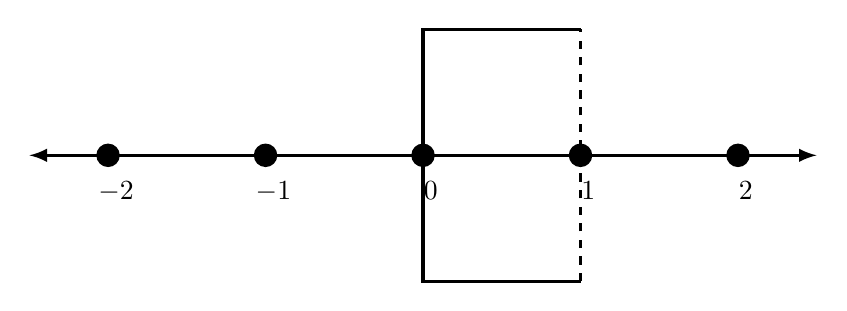
\begin{tikzpicture}[very thick,scale=2]
            \draw[latex-latex] (-2.5,0) -- (2.5,0); 
            \foreach \x in  {-2,-1,0,1,2}
            {
                \node at (\x, 0)[circle,fill,inner sep=3pt]{};
                \draw[shift={(\x+0.05,-0.1)}] node[below] {$\x$};
            }
            \draw[dashed] (1,-0.8) -- (1,0.8);
            \draw (1,0.8) -- (0,0.8) -- (0, -0.8) -- (1, -0.8);
        \end{tikzpicture}}
    \end{center}

    同理,我们可以得到
    \[[1]_R = \{y \in \mathbb{R} \mid (1, y) \in \mathbb{R}\} = \{y \in \mathbb{R} \mid 1 \le y < 2\}\]
    如下图所示:

    \begin{center}
        {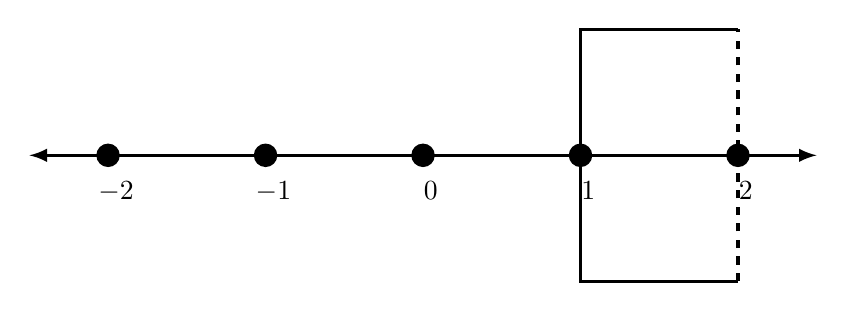
\begin{tikzpicture}[very thick,scale=2]
            \draw[latex-latex] (-2.5,0) -- (2.5,0); 
            \foreach \x in  {-2,-1,0,1,2}
            {
                \node at (\x, 0)[circle,fill,inner sep=3pt]{};
                \draw[shift={(\x+0.05,-0.1)}] node[below] {$\x$};
            }
            \draw[dashed] (2,-0.8) -- (2,0.8);
            \draw (2,0.8) -- (1,0.8) -- (1, -0.8) -- (2, -0.8);
        \end{tikzpicture}}
    \end{center}
\end{example}

请注意,这两个集合是互不相交的,因为第一个集合不包含 $1$,而第二个集合包含 $1$。此外,\emph{每个}实数都\emph{恰好属于一个}这样的区间。例如,我们可以说
\[\pi \in [3]_R, e \in [2]_R, -1.5 \in [-2]_R,\frac{1}{2} \in [0]_R\]
请注意,\emph{等价类}的定义并没有要求我们必须用一个元素来\emph{表示}该类。例如,我们也可以这样说
\[[0]_R = \Big[\frac{1}{2}\Big]_R\]
因为这两个集合是相等的,它们包含相同的元素。任何``向下取整'' 为 $0$ 的实数在 $R$ 下都与 $0$ 相关,因此在 $R$ 下也与 $\frac{1}{2}$ 相关,因为它们的向下取整都是 $0$。

多探索一下这个例子,尝试说服自己,这个划分属性在这里确实有效。在下一部分,我们将在你的帮助下正式证明这一事实的普遍性!由于接下来的讨论会比较抽象,我们建议你多通过实际例子来理解。尝试在另一个集合上定义一个等价关系。它的等价类是什么?你能理解为什么它们会构成一个划分吗?

\subsubsection*{等价类划分集合}

我们已经探讨了等价类\emph{划分}集合的思想,接下来让我们来正式定义这个概念。我们需要先给出一个定义,然后再证明一个定理!这个定理本质上是一个``当且仅当''定理,我们将证明其中一个方向,另一个方向留作练习。

\begin{definition}
    设 $R$ 为集合 $A$ 上的等价关系,关系 $R$ 下等价类的集合记作 $A / R$,即 $A$ \dotuline{模 (modulo)} $R$。也就是说
    \[A / R = \{[x]_R \mid x \in A\}\]
    换种写法是
    \[A / R = \{X \subseteq A \mid \exists x \in A \centerdot X = [x]_R\}\]
\end{definition}

在我们证明重要结果之前,先来看几个例子来理解这些概念。在每个例子中,我们要判断是否存在等价关系,检验等价类,并思考模运算的作用。\\

\begin{example}
    再次考虑定义在实数集 $\mathbb{R}$ 上的关系 $R$ ,其定义为 $(x, y) ∈ R \iff \lfloor x \rfloor = \lfloor y \rfloor$。我们之前已经讨论过为什么这是一个等价关系,现在让我们来研究一下它的等价类。

    根据定义,任何两个相关的元素都有相同的等价类。例如,$[0]_R = [0.5]_R = [0.999]_R$。同样地,$[3.5]_R = [3.75]_R$ ,以及 $[-\pi]_R = [-4]_R$ ,但 $[\pi]_R = [4]_R$。每个实数 $x \in \mathbb{R}$ 都有一个对应的等价类 $[x]_R$,而模运算的思想是通过只考虑必要的等价类来简化 $R$ 的表示。由于 $[0]_R = [0.5]_R = [0.333]_R$ 等等,我们可以用一个集合 $[0]_R$ 来代表所有这些相同的集合。因此,我们可以表示
    \[\mathbb{R} / R = \{\dots, [-2]_R, [-1]_R, [0]_R, [1]_R, [2]_R, \dots \}\]
    实际上,$\mathbb{R} / R$ 可以看作是整数集 $\mathbb{Z}$。然而,我们通常写作 $\mathbb{R} / R ``='' \mathbb{Z}$ 是因为这种等式并不完全准确。特别是,我们还没有严格推导出实数或整数,仅仅严格定义了自然数 $\mathbb{N}$。在这里,我们只是观察到等价类集合与整数集合之间的某种对应关系。我们可以将一个对应到另一个,反之亦然,但这并不意味着它们在技术上是\emph{相等的}。

    不过没关系!这个例子的主要目的是指出 $\mathbb{R} / R$ 是一个等价类的集合。记住,当我们写下一个集合时,顺序和重复是无关紧要的。也就是说, $\{1, 3, 5, 3, 1\}$ 在集合意义上等于 $\{1, 3, 5\}$。它们具有\emph{相同元素},因此是\emph{相同对象}。在当前的上下文中,我们不需要在集合  $\mathbb{R} / R$ 中同时包含 $[0]_R$ 和 $[0.5]_R$,因为它们是同一个对象;在我们的元素列表中重复该对象没有任何意义。

    通常,我们会关注识别等价类的形式并提供一些定性的描述。特别是,我们会经常思考在 $A/R$ 中有多少个等价类。我们还会关注这些类的大小。它们都是一样大的吗?是不是有些类只有几个元素,而有些类则是无穷大的?为什么会这样?这些类元素的``描述''是否大致相同?

    在这个特定的例子中,我们发现 $\mathbb{R} / R$ 中的所有等价类在形式上非常相似。有无限多个等价类 --- 每个整数 $\mathbb{Z}$ 的元素都是一个 --- 它们都是无穷大的,包含一个实数区间。此外,所有这些类的形式都是对于某个 $z \in \mathbb{Z}, [z]_R = \{y \in \mathbb{R} \mid z \le y < z + 1\}$。从这个意义上说,这些等价类都是\emph{性质相似}的。
\end{example}

\begin{example}
    在所有人的集合 $S$ 上定义关系 $B$ 为 $(x, y) \in B \iff x \;\text{和}\; y \;\text{同一个月出生}$。那么 $(\text{欧拉}, \text{庞加莱}) \in B$ 且 $(\text{Paul Erdös}, \text{Emmy Noether}) \in B$。为什么这是等价关系?任何人都与自己相同月份出生(自反性)。如果两个人同一月份出生,那么他们的出生月份是相同的(对称性)。如果 $x$ 和 $y$ 同一月份出生,$y$ 和 $z$ 同一月份出生,那么 $x$ 和 $z$ 也是同一月份出生(传递性)。

    (注意:通常由``有相同的……''或``是相同的……''定义的关系是等价关系。)

    在这个关系下,等价类对应的是月份。因为我们用出生月份来区分人群,一个等价类就是一组同月出生的人。例如,Paul Erdös 和 Emmy Noether 都是三月出生,所以我们可以说 $\text{Emmy Noether} \in [\text{Paul Erdös}]_B$ 这个等价类。这个等价类\emph{对应于}三月,但请注意,它是根据集合 $S$ (所有人)中的特定元素定义的。

    如果我们定义 $M$ 为所有三月出生的人的集合,那么我们可以说 $M = [\text{Paul Erdös}]_B$。综合这些观察,我们可以得出结论:按出生月份划分人的集合,记为 $S/B$,由 $12$ 个集合组成,每个集合对应一个不同月份,并包含所有在那个月份出生的人。
\end{example}

\begin{example}
    考虑所有有序实数对的集合 $\mathbb{R} \times \mathbb{R}$。我们通过定义两个对何时\emph{相关}来定义 $\mathbb{R} \times \mathbb{R}$ 上的关系 $R$。具体来说,我们定义
    \[\big((x, y),(u, v)\big) \in R \iff x = u\]
    也就是说,当平面上的两点第一个坐标相同时,它们在关系 $R$ 下是相关的。想想为什么这是一个等价关系?从几何上讲,这个关系只关心一个点所在的垂直于 $y$ 轴的直线。理解这一点后,你可以很容易地``看出''并解释为什么 $R$ 是一个等价关系,而严格证明这一点只需要多写一些内容和符号。(试试看!)

    这也使我们能够轻松描述和可视化这个关系下的等价类。所有在同一垂线上的点都属于同一个等价类,我们可以通过查看这些垂线与水平轴的交点来索引这些类。例如,$(1, 3) \in [(1, 0)]_R$,因为点 $(1, 3)$ 和 $(1, 0)$ 位于同一条垂线上。我们可以用这种方式表示\emph{每一个}等价类:$[(x, 0)]_R$,其中 $x \in \mathbb{R}$。
\end{example}

\begin{center}
    {\begin{tikzpicture}[very thick,scale=2]
        \draw[latex-latex] (-1.5,0) -- (2.5,0); 
        \draw[latex-latex] (0,-1.5) -- (0,3.5); 
        \foreach \x in  {1,2}
        {
            \node at (\x, 0)[circle,fill,inner sep=3pt]{};
            \draw[shift={(\x+0.25,-0.1)}] node[below] {$(\x, 0)$};
        }
        \foreach \y in  {1,2,3}
        {
            \node at (0, \y)[circle,fill,inner sep=3pt]{};
            \draw[shift={(-0.15, \y)}] node[left] {$(0, \y)$};
        }
        \draw[dashed] (1,-1.5) -- (1,3.5);
        \node at (1, 3)[circle,fill,inner sep=3pt]{};
        \draw[shift={(1.15, 3)}] node[right] {$(1, 3)$};
        \draw[shift={(1.15, 1.5)}] node[right] {$[(1,0)]_R = \{(1, y)\}$};
    \end{tikzpicture}}
\end{center}

因此,在某种意义上,等价类的集合 $(\mathbb{R} \times \mathbb{R})/R$ 与实数轴 $\mathbb{R}$ 是``等同的''!通过忽略第二个坐标,我们可以将平面上的所有点压缩到水平轴上。从数学上讲,有一种方法可以更精确地表达这个想法,但在此我们无法正式讨论。简单来说,$\mathbb{R} \times \mathbb{R}$ 上的这个关系产生的等价类由 $\mathbb{R}$ 表示,这其中存在一些有趣的现象。

这里有另一个 $\mathbb{R} \times \mathbb{R}$ 上的关系。定义 $S$ 为
\[\big((x, y),(u, v)\big) \in S \iff \sqrt{x^2+y^2} = \sqrt{u^2+v^2}\]
回想一下基本的几何和代数知识,你可能会发现表达式 $\sqrt{x^2 + y^2}$ 描述的是点 $(x, y)$ 到原点 $(0, 0)$ 的距离。(在数学中,我们称这种表达式为\emph{度量 (metric)}。)因此,这个关系表明,当两点到原点的距离相同时,它们是等价的。从视觉上来看,这解释了为什么 $S$ 是一个等价关系,并且展示了等价类是以原点为中心的圆。因此,我们可以通过这些圆的一个显著特征 --- 它们的\emph{半径} $r \ge 0$,来描述集合 $(\mathbb{R} \times \mathbb{R})/S$ 的元素。因此,在 $S$ 下的等价类集合与非负实数集合是``等同的''!

\begin{center}
    {\begin{tikzpicture}[very thick,scale=2]
        \draw[latex-latex] (-3,0) -- (3,0); 
        \draw[latex-latex] (0,-3) -- (0,3); 
        \foreach \x in  {-2,-1,0,1,2}
        {
            \node at (\x, 0)[circle,fill,inner sep=3pt]{};
            \node at (0, \x)[circle,fill,inner sep=3pt]{};
        }
        \draw[dashed] (0,0) circle (1);
        \draw[dashed] (0,0) circle (2);
        \draw[shift={(0.8, -0.7)}] node[right] {$[(1,0)]_S$};
        \draw[shift={(0.8, -0.9)}] node[right] {$r=1$};
        \draw[shift={(1.7, 1.5)}] node[right] {$[(2,0)]_S$};
        \draw[shift={(1.7, 1.3)}] node[right] {$r=2$};
    \end{tikzpicture}}
\end{center}

这听起来有点奇怪,对吧?我们从一个二维集合开始,关联成对的点,并整理出等价类,结果得到了一个一维集合。(注意:我们这里还没有正式的方法来定义\emph{维度},但你应该能理解我们的意思。)回顾一下上面在 $\mathbb{R}^2$ 上定义的关系 $R$。如果我们只在 $\mathbb{R}^2$ 的``右半部分''定义这个关系,也就是所有第一个坐标非负的点,那么等价类的集合也会和非负实数集合``相同''。从哪个角度看,这个集合和 $(\mathbb{R} \times \mathbb{R})/S$ 是``相同''的呢?这个问题合理吗?我们该如何\emph{证明}此说法?这些都是非常有趣的问题,我们鼓励你思考一下这些问题!

不要过于纠结于这些概念和问题。关键在于:等价类的集合构成底层集合的\textbf{划分}。

现在我们已经看过了若干例子,接下来我们来陈述(并证明!)一些关于等价关系的重要结论。主要是,这些定理说明了我们一直暗示的观点,即等价关系会将集合划分成相应的等价类。不过,令人惊讶的是,我们还有一个有趣的结论:给定任意一个划分,我们可以为其定义一个等价关系!

\begin{theorem}\label{theorem6.4.10}
    设 $R$ 为集合 $A$ 上的等价关系。则属于 $A/R$ 的集合构成 $A$ 的划分。也就是说,它们是非空的,互不相交的,它们的并集是 $A$。
\end{theorem}

\begin{proof}
    见习题 \ref{exc:exercises6.7.13}
\end{proof}

我们将在本章末尾的习题 \ref{exc:exercises6.7.13} 中带你完成这个结论的证明。我们之前研究的例子应该可以帮助你直观地理解为什么这个定理是正确的,而通过详细地推导证明过程,你将对其背后的数学严谨性有一个扎实的理解。

\subsubsection*{划分产生等价关系}

现在,我们来看一个类似且重要的结论,这是前一个定理的逆命题。为了更好地理解这个定理,我们先看一个例子,这个例子还将为我们提供定理证明的概要。\\

\begin{example}
    考虑集合 $S=[6]$。定义集合
    \[\mathcal{F} = \{ \{1, 4\}, \{2, 3, 5\} , \{6\} \}\]
    注意,$\mathcal{F}$ 是 $S$ 的一个划分,因为这些集合是互不相交的,非空的,且它们的并集是 $S$。如果有一种等价关系 $R$,使得我们在考虑 $S/R$ 时得到这些集合,那不是很好吗?事实上,确实存在这样的关系!尽管我们可能无法像之前那样,以一种优雅的方式定义它们,例如通常的``$(x, y) \in R \iff x \;\text{和}\; y \;\text{具有某种共同属性}$''。不过,既然我们已经有了划分,就可以用它来定义关系。具体来说,划分集合就是等价类。划分本身建立了等价类的结构,我们只需通过 $(x, y) \in R \iff x \;\text{和}\; y \;\text{属于同一个划分集合}$ 来定义等价关系 $R$。

    在本例中,我们可以定义 $S_1 = \{1, 4\} , S_2 = \{2, 3, 5\} , S_3 = \{6\}$,则我们可以定义 $R$
    \[(x, y) \in R \iff \exists i \in [3] \centerdot (x \in S_i \land y \in S_i)\]
\end{example}

想一想为什么这种方法有效。你能理解为什么这是一个等价关系吗?你知道等价类是什么吗?

现在我们准备陈述并证明这个定理。

\begin{theorem}\label{theorem6.4.12}
    设 $S$ 为集合,并设 $\mathcal{F}$ 为集合 $S$ 的划分。则存在等价关系 $R$ 使得 $S/R=\mathcal{F}$。
\end{theorem}

正如我们之前提到的,这个结果完全依赖于一个事实:划分是一组集合,这些集合正是我们要定义的等价类。我们只需要证明``$x$ 和 $y$ 相关当且仅当 $x$ 和 $y$ 属于同一个划分集合''这个关系是一个等价关系。这并不难!在阅读我们的证明之前,试着自己勾画一下证明的细节吧!

\begin{proof}
    设 $\mathcal{F}$ 为集合 $S$ 的划分。这意味着我们有一个索引集 $I$,且
    \[\mathcal{F} = {S_i \mid i \in I}\]
    其中集合 $S_i$ 满足 $S_i \subseteq S$ 且 $S_i \ne \varnothing$ 且
    \[\bigcup_{i \in I} S_i = S \quad \text{且} \quad \forall i, j \in I \centerdot i \ne j \implies S_i \cap S_j = \varnothing\]
    定义 $S$ 上的关系 $R$ 为
    \[(x, y) \in R \iff \exists i \in I \centerdot (x \in S_i \land y \in S_i)\]
    我们要证明 $R$ 是等价关系。

    \begin{itemize}
        \item 设 $x \in S$ 是任意固定的。由于 $S_i$ 的集合覆盖 $S$,因此我们知道 $\exists i \in I \centerdot x \in S_i$。给定这样的 $i$,则必然有 $x \in S_i$ 且 $x \in S_i$,所以 $(x,x) \in R$。因此 $R$ 具有自反性。
        \item 设 $x, y \in S$ 是任意固定的。假设 $(x, y) \in R$。这意味着 $\exists i \in I \centerdot (x \in S_i \land y \in S_i)$。给定这样的 $i$,则必然有 $y \in S_i \land x \in S_i$,所以 $(y,x) \in R$。因此 $R$ 具有对称性。
        \item 设 $x, y, z \in S$ 是任意固定的。假设 $(x, y) \in R$ 且 $(y, z) \in R$。这意味着 $\exists i \in I \centerdot (x \in S_i \land y \in S_i)$ 且 $\exists j \in I \centerdot (y \in S_j \land z \in S_j)$。给定这样的 $i,j$,注意 $y \in S_i \land y \in S_j$,而对于任意不同的 $i,j, S_i \cap S_j = \varnothing$,因此 $i=j$(否则会出现 $y \in \varnothing$,而这是不可能的!)由于 $x \in S_i, y \in S_i, z \in S_i$,所以 $(x,z) \in R$。因此 $R$ 具有传递性。
    \end{itemize}
    由于上面三个性质成立,所以 $R$ 是一个等价关系!

    $S/R$ 的等价类写做 $[x]_R$,其中 $x \in S$。因为 $\mathcal{F}$ 是 $A$ 的分割,对于某个 $i, x \in S_i$,所以对于某个 $i, [x]_R = S_i$。因此所有等级类等于某集合 $S_i$。

    类似地,任意集合 $S_i \ne \varnothing$,所以 $\exists x \in S_i$,因此存在对应的等价类 $S_i=[x]_R$。因此,每个等价类都是形如 $S_i$ 的集合,反之亦然。
\end{proof}

这表明,任何划分都可以很好地对应一个等价关系及其等价类!

\subsection{更多示例}

现在我们已经掌握了这两个定理,让我们通过一些关系的例子来进一步理解它们。对于每个例子,我们将尝试判断它是否是等价关系。如果是,我们可以描述它的等价类。如果不是,我们可以参考其中一个定理,看看为什么它不是等价关系。\\

\begin{example}
    我们先从一个简单的例子开始。回顾一下我们在示例 \ref{ex:example6.2.9} 中定义的等式关系。我们已经解释过,``$=$'' 在任何集合上都是等价关系。具体来说,它将一个集合划分为等价类,而这些等价类正是集合的各个元素本身。例如,在集合 $\mathbb{N}$ 中,$[1]_{=} = \{1\}, [2]_{=} = \{2\}$,以此类推。所有的等价类都是\emph{单例的}(集合只有一个元素)。
\end{example}

\begin{example}
    我们再来看一个相对简单的例子。回顾一下我们在示例 \ref{ex:example6.2.5} 中定义的 $\mathbb{Z}$ 集合上的奇偶关系。这是一个等价关系,现在让我们来证明这一点。
    \begin{proof}
        设 $a, b, c \in \mathbb{Z}$ 是任意的。

        首先,不难发现 $(a,a) \in R$ 因为 $a$ 与其自身有相同的奇偶性。因此 $R$ 具有自反性。

        其次,假设 $(a,b) \in R$,所以 $a$ 和 $b$ 具有相同的奇偶性。那么显然 $b$ 和 $a$ 也具有相同的奇偶性,所以 $(b,a) \in R$。因此 $R$ 具有对称性。

        最后,假设 $(a,b) \in R$ 且 $(b,c) \in R$。如果 $a$ 是奇数,我们可以推导出 $b$ 为奇数且 $c$ 也为奇数;同理,如果 $a$ 为偶数,我们可以推导出 $b$ 为偶数且 $c$ 也为偶数。无论是哪种情况,$a$ 和 $c$ 都具有相同的奇偶性,所以必然有 $(a,c) \in R$。因此 $R$ 具有传递性。

        因为 $R$ 具有自反性、对称性和传递性,所以 $R$ 是一个等价关系。
    \end{proof}

    这意味着等价类集合 $\mathbb{Z}/R$ 构成 $\mathbb{Z}$ 的划分。现在让我们来确定该划分。

    考虑 $[0]_R$,这是所有与 $0$ 奇偶性相同的整数集合,即所有\emph{偶数}。因此,在这种情况下,
    \[\mathbb{Z}/R = \{O_{\mathbb{Z}}, E_{\mathbb{Z}}\}\]
    其中 $O_{\mathbb{Z}}$ 是奇数集,$E_{\mathbb{Z}}$ 是偶数集。这两个等价类都是无穷大的。
\end{example}

\begin{example}
    回顾我们在示例 \ref{ex:example6.2.6} 中定义的 $\mathbb{R}$ 上的顺序关系。这个关系是等价关系吗?我们可以通过检查定义中的每个属性来确定。要注意的是,无论 $x$ 是什么,只要 $x \in \mathbb{R}$,就有 $(x, x) \notin R$,因为 $x \nless x$。因此,$R$ 不具有自反性,所以它不是等价关系。(另外,$R$ 也不具有对称性,但它具有传递性。)

    为什么严格的顺序关系不会是等价关系呢?为什么我们希望等价关系是自反的?想想\emph{等价类}的概念;等价关系应该把整个集合的元素划分成几部分,我们可以通过属于某部分的一个元素来识别这部分。对于非自反的关系,有些元素不属于它们自己的``等价类'',这显然是不理想的!

    (后续问题:对于自反的顺序关系 $\le$,它是等价关系吗?为什么是或者为什么不是?)
    
    换句话说,$\mathbb{R}$ 上的 ``$<$'' 关系并没有把实数划分为几部分。基于这一点,并结合定理 \ref{theorem6.4.10} 的\emph{逆否}命题,我们可以得出 ``$<$'' \emph{不是}一个等价关系。
\end{example}

\begin{example}
    定义 $\mathbb{R} \times \mathbb{R}$ 上的关系 $\sim$ 为
    \[(x, y) \sim (u, v) \iff x \le u \land y \le v\]
    即使不检查其具体属性,我们也可以尝试判断它是否是等价关系。为此,我们选取集合中的一个特定元素,并查看与该特定元素相关的所有元素。在下图中,我们使用 $(1, 1)$ 作为这个特定元素。

    \begin{center}
        {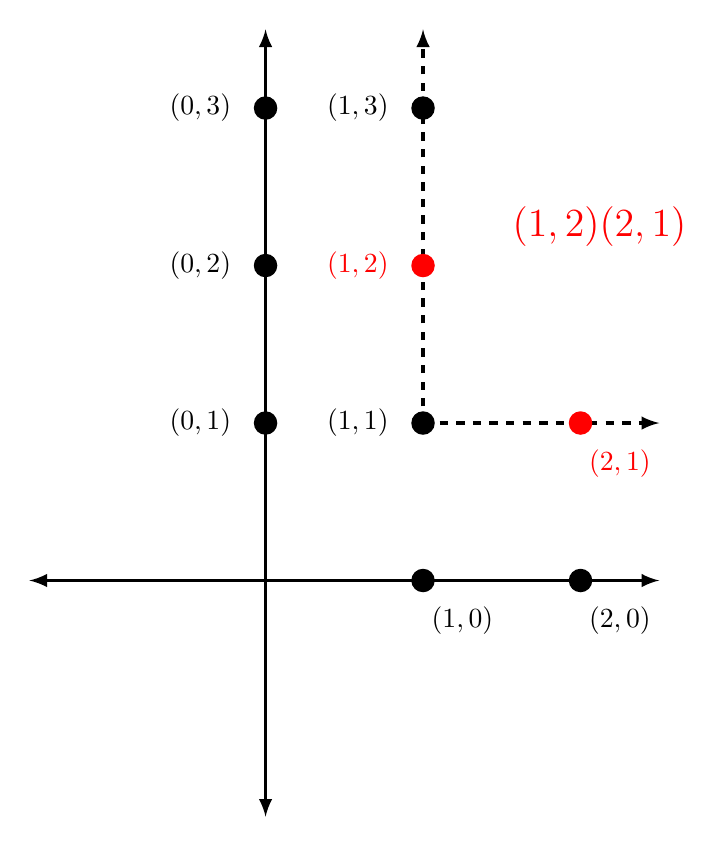
\begin{tikzpicture}[very thick,scale=2]
            \draw[latex-latex] (-1.5,0) -- (2.5,0); 
            \draw[latex-latex] (0,-1.5) -- (0,3.5); 
            \foreach \x in  {1,2}
            {
                \node at (\x, 0)[circle,fill,inner sep=3pt]{};
                \draw[shift={(\x+0.25,-0.1)}] node[below] {$(\x, 0)$};
                
            }
            \foreach \y in  {1,2,3}
            {
                \node at (0, \y)[circle,fill,inner sep=3pt]{};
                \draw[shift={(-0.15, \y)}] node[left] {$(0, \y)$};
            }
    
            \draw[dashed,-latex] (1,1) -- (2.5,1); 
            \draw[dashed,-latex] (1,1) -- (1,3.5); 
            \foreach \y in  {1,3}
            {
                \node at (1, \y)[circle,fill,inner sep=3pt]{};
                \draw[shift={(0.85, \y)}] node[left] {$(1, \y)$};
            }
    
            \node[red] at (1, 2)[circle,fill,inner sep=3pt]{};
            \draw[color=red, shift={(0.85, 2)}] node[left] {$(1, 2)$};
            \node[red] at (2, 1)[circle,fill,inner sep=3pt]{};
            \draw[color=red, shift={(2.25, 0.9)}] node[below] {$(2, 1)$};
    
            \draw[color=red, font=\Large, shift={(1.5, 2.25)}] node[right] {$(1,2) \nsim (2,1)$};
        \end{tikzpicture}}
    \end{center}

    请注意,$\sim$ 的定义条件要求一个点必须位于另一个点的``右上方''才能使两者相关。同时,不等式是``$\le$'',因此第二个点不必\emph{严格}位于上方或右侧。

    因此,我们可以从上图看到,$(1, 2) \sim (1, 1)$(因为 $1 \le 1$ 且 $1 \le 2$)。同理,$(1, 1) \sim (2, 1)$。因此,点 $(1, 2)$ 和 $(2, 1)$ 都与 $(1, 1)$ 相关。为了使 $\sim$ 成为\emph{等价关系},我们需要 $(2, 1$) 和 $(1, 2)$ 也彼此相关。因为它们必须同属于 $(1, 1)$ 的``等价类''。然而,遗憾的是,$(1, 2) \nsim (2, 1)$。第二个点严格位于第一个点的``左下方'',因此不满足 $\sim$ 的定义条件。

    这意味着所有与 $(1, 1)$ 相关的元素的集合\textbf{不能}形成一个``封闭集合''。从数学上讲,这些元素的集合不是一个等价类。因此,$\sim$ \textbf{不是}一个等价关系。

    现在,试着识别 $\sim$ 具有哪些性质和不具备哪些性质。它具有自反性吗?具有对称性吗?具有传递性吗?为什么具有或者为什么不具有?通过这样做,你会再次证明 $\sim$ 不是一个等价关系。事先弄清楚这一点,是不是很有帮助呢?我们建议,当你遇到一个定义好的关系时,可以做类似的分析。你能找出``等价类''可能是什么吗?如果能,那么你对这个关系为何以及如何是等价关系有了一些直觉,这将帮助你描述等价类。如果不能,那么你也会对如何反驳这种说法有一些理解。
\end{example}

\subsubsection*{[选学] $\mathbb{Z}$ 是如何从 $\mathbb{N} \times \mathbb{N}$ 上的等价关系生成的}

还记得第 \ref{ch:chapter03} 章中的那个复杂习题吗?它要求你证明某些关于自然数对的性质,并声称这是在证明整数的存在性。那到底是怎么回事呢?现在回头看看习题 \ref{exc:exercises3.11.22}。你会发现问题的最后三个部分要求你证明我们定义的集合 $R$ 是集合 $P$ 上的\textbf{等价关系}(底层集合是 $P = \mathbb{N} \times \mathbb{N}$)。好好看一下!你已经证明了 $R$ 具有自反性、对称性和传递性。

这个练习表明(在这里我们略过了一些细节)任何负整数都可以表示为两个整数之差为该负整数的\textbf{等价类}。也就是说
\[-1 \;\text{``$=$''}\; [(1, 2)]_R = \{(1, 2),(2, 3),(3, 4), \dots \}\]
再比如
\[-3 \;\text{``$=$''}\; [(1, 4)]_R = \{(1, 4),(2, 5),(3, 6), \dots \}\]
这只是一个直观的解释,从数学上讲并不严格,但这就是主要思路!

\subsection{习题}

\subsubsection*{温故知新}

以口头或书面的形式简要回答以下问题。这些问题全都基于你刚刚阅读的内容,所以如果忘记了具体的定义、概念或示例,可以回去重读相关部分。确保在继续学习之前能够自信地回答这些问题,这将有助于你的理解和记忆!

\begin{enumerate}[label=(\arabic*)]
    \item \emph{等价关系}需要满足哪些性质?
    \item 什么是等价类?等价类中的所有元素必须满足什么条件?
    \item 给定集合 $S$ 和 $S$ 上的等价关系 $R$,等价类的集合必须满足什么条件?
\end{enumerate}

\subsubsection*{小试牛刀}

尝试回答以下问题。这些题目要求你实际动笔写下答案,或(对朋友/同学)口头陈述答案。目的是帮助你练习使用新的概念、定义和符号。题目都比较简单,确保能够解决这些问题将对你大有帮助!

\begin{enumerate}[label=(\arabic*)]
    \item 回顾 \ref{sec:section6.2.5} 节习题 \ref{exc:exercises6.2.2} 中定义的关系。我们在该习题中定义 $\mathbb{Z}$ 上的关系 $\bigstar$ 为
    \[\forall x, y \in \mathbb{Z} \centerdot x \;\bigstar\; y \iff 3 \mid x - y\]
    你之前已经证明了它确实是一个等价关系。现在,请描述一下 $\mathbb{Z}/\bigstar$ 的等价类。有多少个等价类?每个等价类有多大?你能列出它们的元素或描述它们的特征吗?
    \item 回顾 \ref{sec:section6.2.5} 节习题 \ref{exc:exercises6.2.3} 中定义的关系。我们在该习题中定义 $\mathbb{Z}$ 上的关系 $\sim$ 为
    \[\forall x, y \in \mathbb{Z} \centerdot x \sim y \iff 3 \mid x + 2y\]
    你之前已经证明了它确实是一个等价关系。现在,请判别并描述 $\mathbb{Z}/\sim$ 的等价类。有多少个等价类?每个等价类有多大?你能列出它们的元素或描述它们的特征吗?对比上一题,你有什么发现?
    \item 考虑集合 $[5]=\{1,2,3,4,5\}$。定义 $[5]$ 上的关系 $\approx$ 为,对于任意 $x,y \in [5]$
    \[x \approx y \iff \vert x^2 - y^2 \vert \le 5\]
    对于任意 $x \in [5]$,设 $S(x)$ 为满足 $x \approx y$ 且 $y \in [5]$ 的所有元素的集合。
    \begin{enumerate}[label=(\alph*)]
        \item 写出集合 $S(1), S(2), S(3), S(4), S(5)$ 的所有元素。
        \item 通过观察这些集合,你能判断 $\approx$ 是否是一个等价关系吗?你是怎么判断的?
        \item 通过证明或证伪自反性、对称性和传递性,来证明 $\approx$ 是否是一个等价关系。
    \end{enumerate}
    \item 考虑集合 $\mathbb{N} \times \mathbb{N}$。定义该集合上的关系 $\sim$ 为
    \[(a, b) \sim (c, d) \iff a + b = c + d\]
    判断该关系否是一个等价关系。如果是,请可视化地描述其等价类。
\end{enumerate}